\section{Reengineered Task Organization Model}
Das Reengineered Task Organization Model repräsentiert die Arbeit der Benutzer mithilfe des zu entwicklende System. Die Abbildung \ref{img:reengineeredTaskOrganizationModel}: \nameref{img:reengineeredTaskOrganizationModel} beschreibt den Prozess der Arbeit des Diabetikers mit dem System anhand der Concrete Use Cases aus der Aufgebenmodellierung und ergänzt das Task Organization Model.
\begin{figure}[H]
	\centering
	\setlength{\fboxsep}{1pt}
	\setlength{\fboxrule}{1pt}
	\fbox{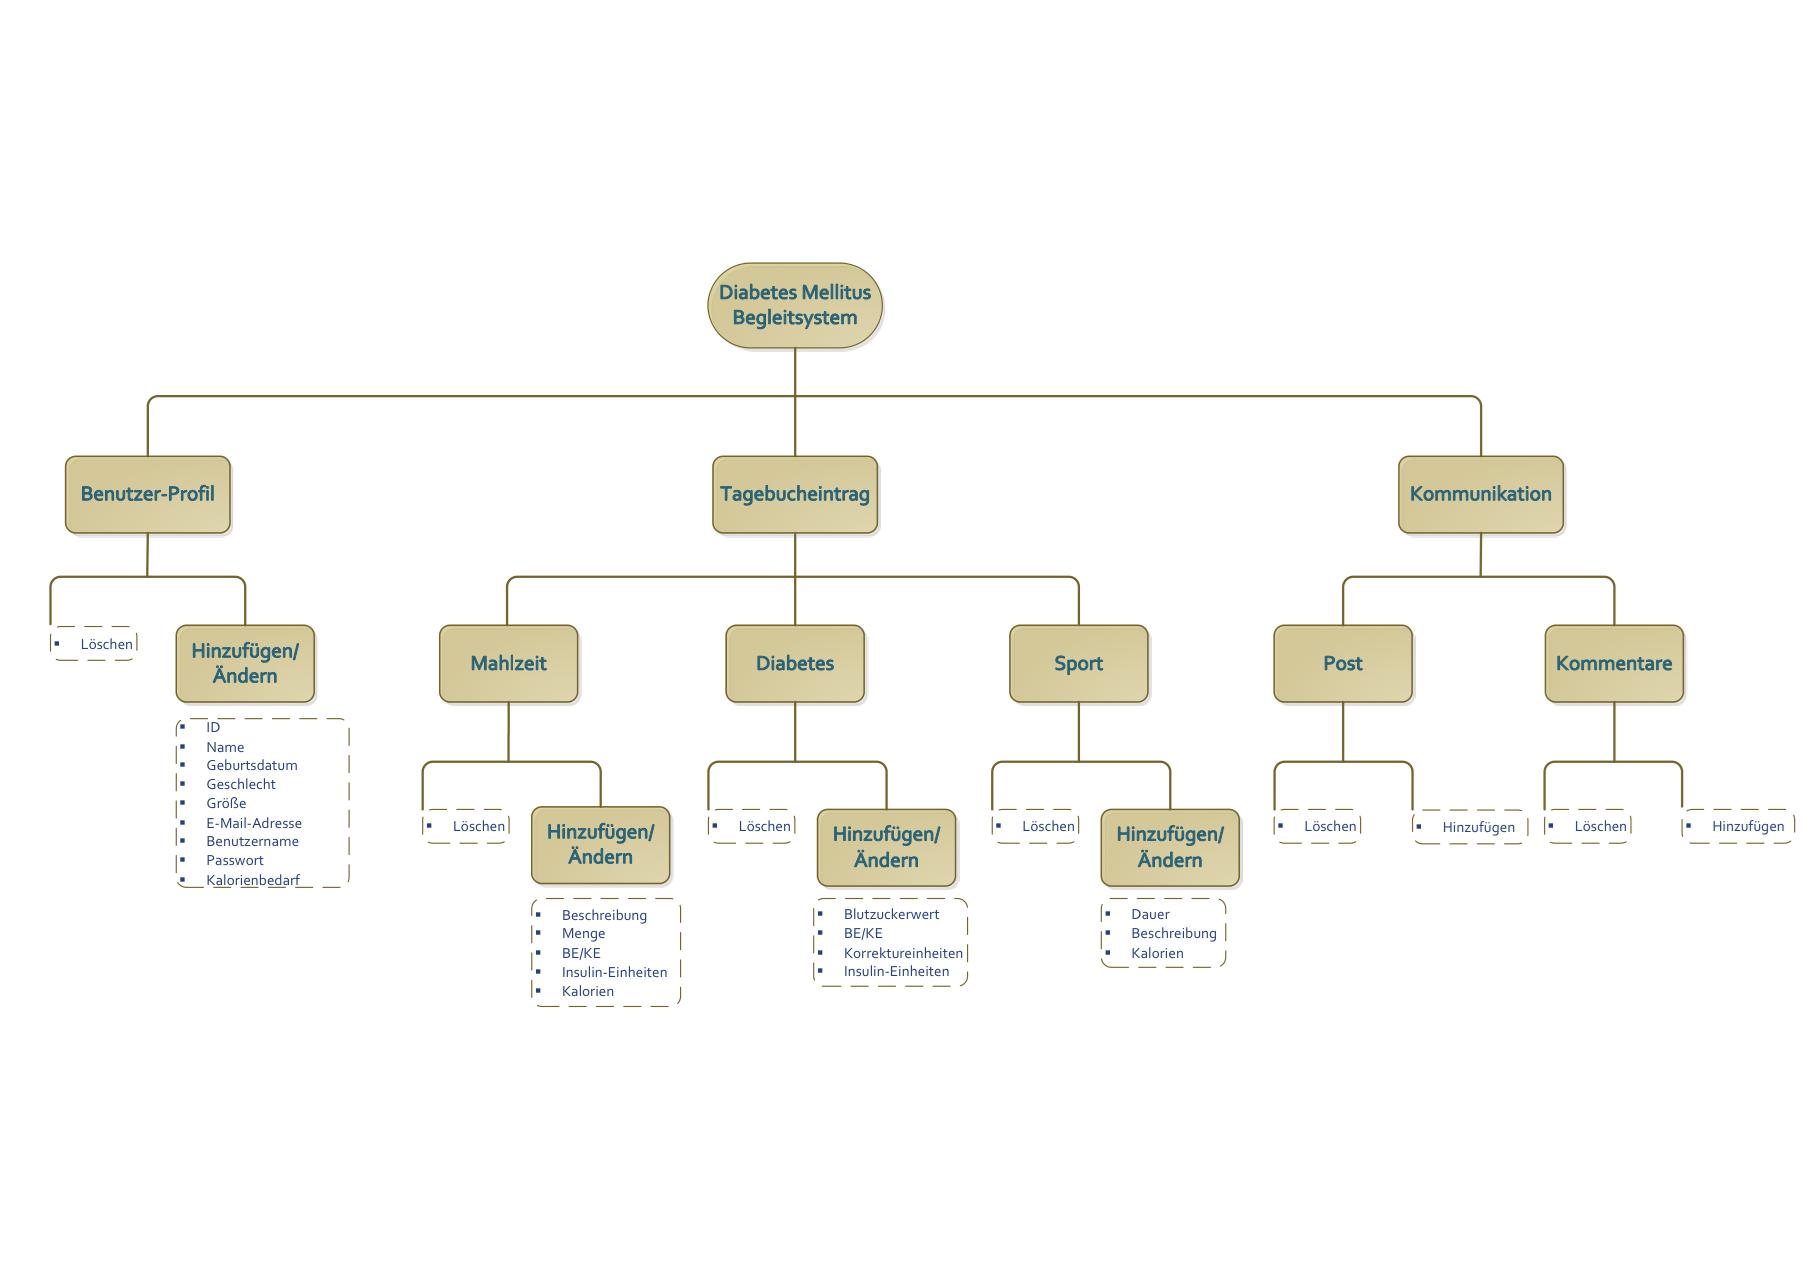
\includegraphics[width=1.0\textwidth]{images/reengineeredTaskOrganizationModel.png}}
	\captionsetup{justification=centering}
	\caption{Reengineered Task Organization Model}
	\label{img:reengineeredTaskOrganizationModel}
\end{figure}